\documentclass[11pt]{article}
\usepackage{aclsub}
\usepackage{graphicx}

\title{Advances in domain independent linear text segmentation}
\id{NAACL-126}
\area{Discourse; Corpus-Based NLP}
\keywords{Linear text segmentation}
\whichconference{NAACL}
\wordcount{2400}
\otherconferences{none}
\summary{This paper describes a method for linear text segmentation which is twice as accurate and over seven times as fast as the current state-of-the-art. Inter-sentence similarity is replaced by rank in the local context. Boundary locations are discovered by clustering.}

%\author{Freddy Y. Y. Choi\\Artificial Intelligence Group\\Department of Computer Science\\University of Manchester\\Oxford Road, Manchester\\England\\choif@cs.man.ac.uk}

\begin{document}
\maketitle

\section{Introduction}
Even moderately long documents typically address several topics or different aspects of the same topic. The aim of linear text segmentation is to discover the topic boundaries. The uses of this procedure include information retrieval \cite{hearst_1994,yaari_1997,reynar_1999}, summarization \cite{reynar_1998}, text understanding \cite{kozima_1993}, language modelling \cite{morris_hirst_1991,beeferman_et_al_1997} and in our case, improving the efficiency of screen readers for the visually disabled.

In \cite{reynar_1998}, Reynar shows that his optimization algorithm is the state-of-the-art algorithm for domain independent linear text segmentation. Although recent work \cite{reynar_1999,beeferman_et_al_1999} demonstrates accuracy can be improved by combining multiple information sources, the performance gain stems from the use of domain specific features such as cue phrases. This paper focuses on domain independent algorithms for text segmentation.

\section{Background}
Existing methods for detecting topic boundaries fall into one of two categories, lexical cohesion methods and multi-source methods \cite{yaari_1997}. The former stems from the work of Halliday and Hasan \cite{halliday_hasan_1976}. They proposed that text segments with similar vocabulary are likely to be part of a coherent topic segment. Implementations of this idea use word stem repetition \cite{reynar_1994,ponte_croft_1997}, context vectors \cite{hearst_1994,yaari_1997,kaufmann_1999,eichmann_et_al_1999}, entity repetition \cite{kan_et_al_1998}, semantic similarity \cite{morris_hirst_1991,kozima_1993}, word distance model \cite{beeferman_et_al_1997b} and word frequency model \cite{reynar_1999} to detect cohesion. Methods for finding the location of topic boundaries include sliding window \cite{hearst_1994}, lexical chains \cite{morris_1988,kan_et_al_1998}, agglomerative clustering \cite{yaari_1997} and dot-plotting, or divisive clustering \cite{reynar_1994}. Lexical cohesion methods are typically used for segmenting text documents in a collection to improve information retrieval \cite{hearst_1994,reynar_1998}.

Multi-source methods combine lexical cohesion with other indicators of topic shift such as cue phrases, prosodic features, reference, syntax and lexical attraction \cite{beeferman_et_al_1997b} using decision trees \cite{litman_passonneau_1995} and probabistic models \cite{beeferman_et_al_1997,reynar_1998}. These methods are generally used for segmenting transcribed spoken text such as news broadcast where the presentation format and the use of topic shift cues are predictable.

\section{Algorithm}
Our segmentation algorithm takes a list of tokenized sentences as input. A tokenizer \cite{grefenstette_1994} and a sentence boundary disambiguation algorithm \cite{palmer_hearst_1994,reynar_ratnaparkhi_1997} are used to convert a plain text document into the acceptable input format. 

\subsection{Similarity measure}
Punctuations and uninformative words are removed from each sentence using a simple regular expression pattern matcher and a stopword list. A stemming algorithm \cite{porter_1980} is then applied to the remaining tokens to obtain the word stems. A dictionary of word stem frequencies is constructed for each sentence. This is represented as a vector of frequency counts.

Let $f_{i,j}$ denote the frequency of word $j$ in sentence $i$. The similarity between a pair of sentences $x,y$ is computed using the cosine measure \cite{hearst_1994} shown in equation \ref{eq:cosine}. This is applied to all sentence pairs to generate a similarity matrix.
\begin{equation}
sim(x,y) = \frac{\sum_{j} f_{x,j} \times f_{y,j}}{\sqrt{{\sum_{j} f_{x,j}^2} \times {\sum_{j} f_{y,j}^2}}}
\label{eq:cosine}
\end{equation}

Figure \ref{fig:simmatrix} shows an example of a similarity matrix\footnote{The contrast of the image has been adjusted to highlight the image features. }. High similarity values are represented by bright pixels. The bottom-left and top-right pixel show the self-similarity for the first and last sentence, respectively. Notice the matrix is symmetric and contains bright square regions along the diagonal. These represent cohesive text segments.

\begin{figure}[h]
\begin{center}
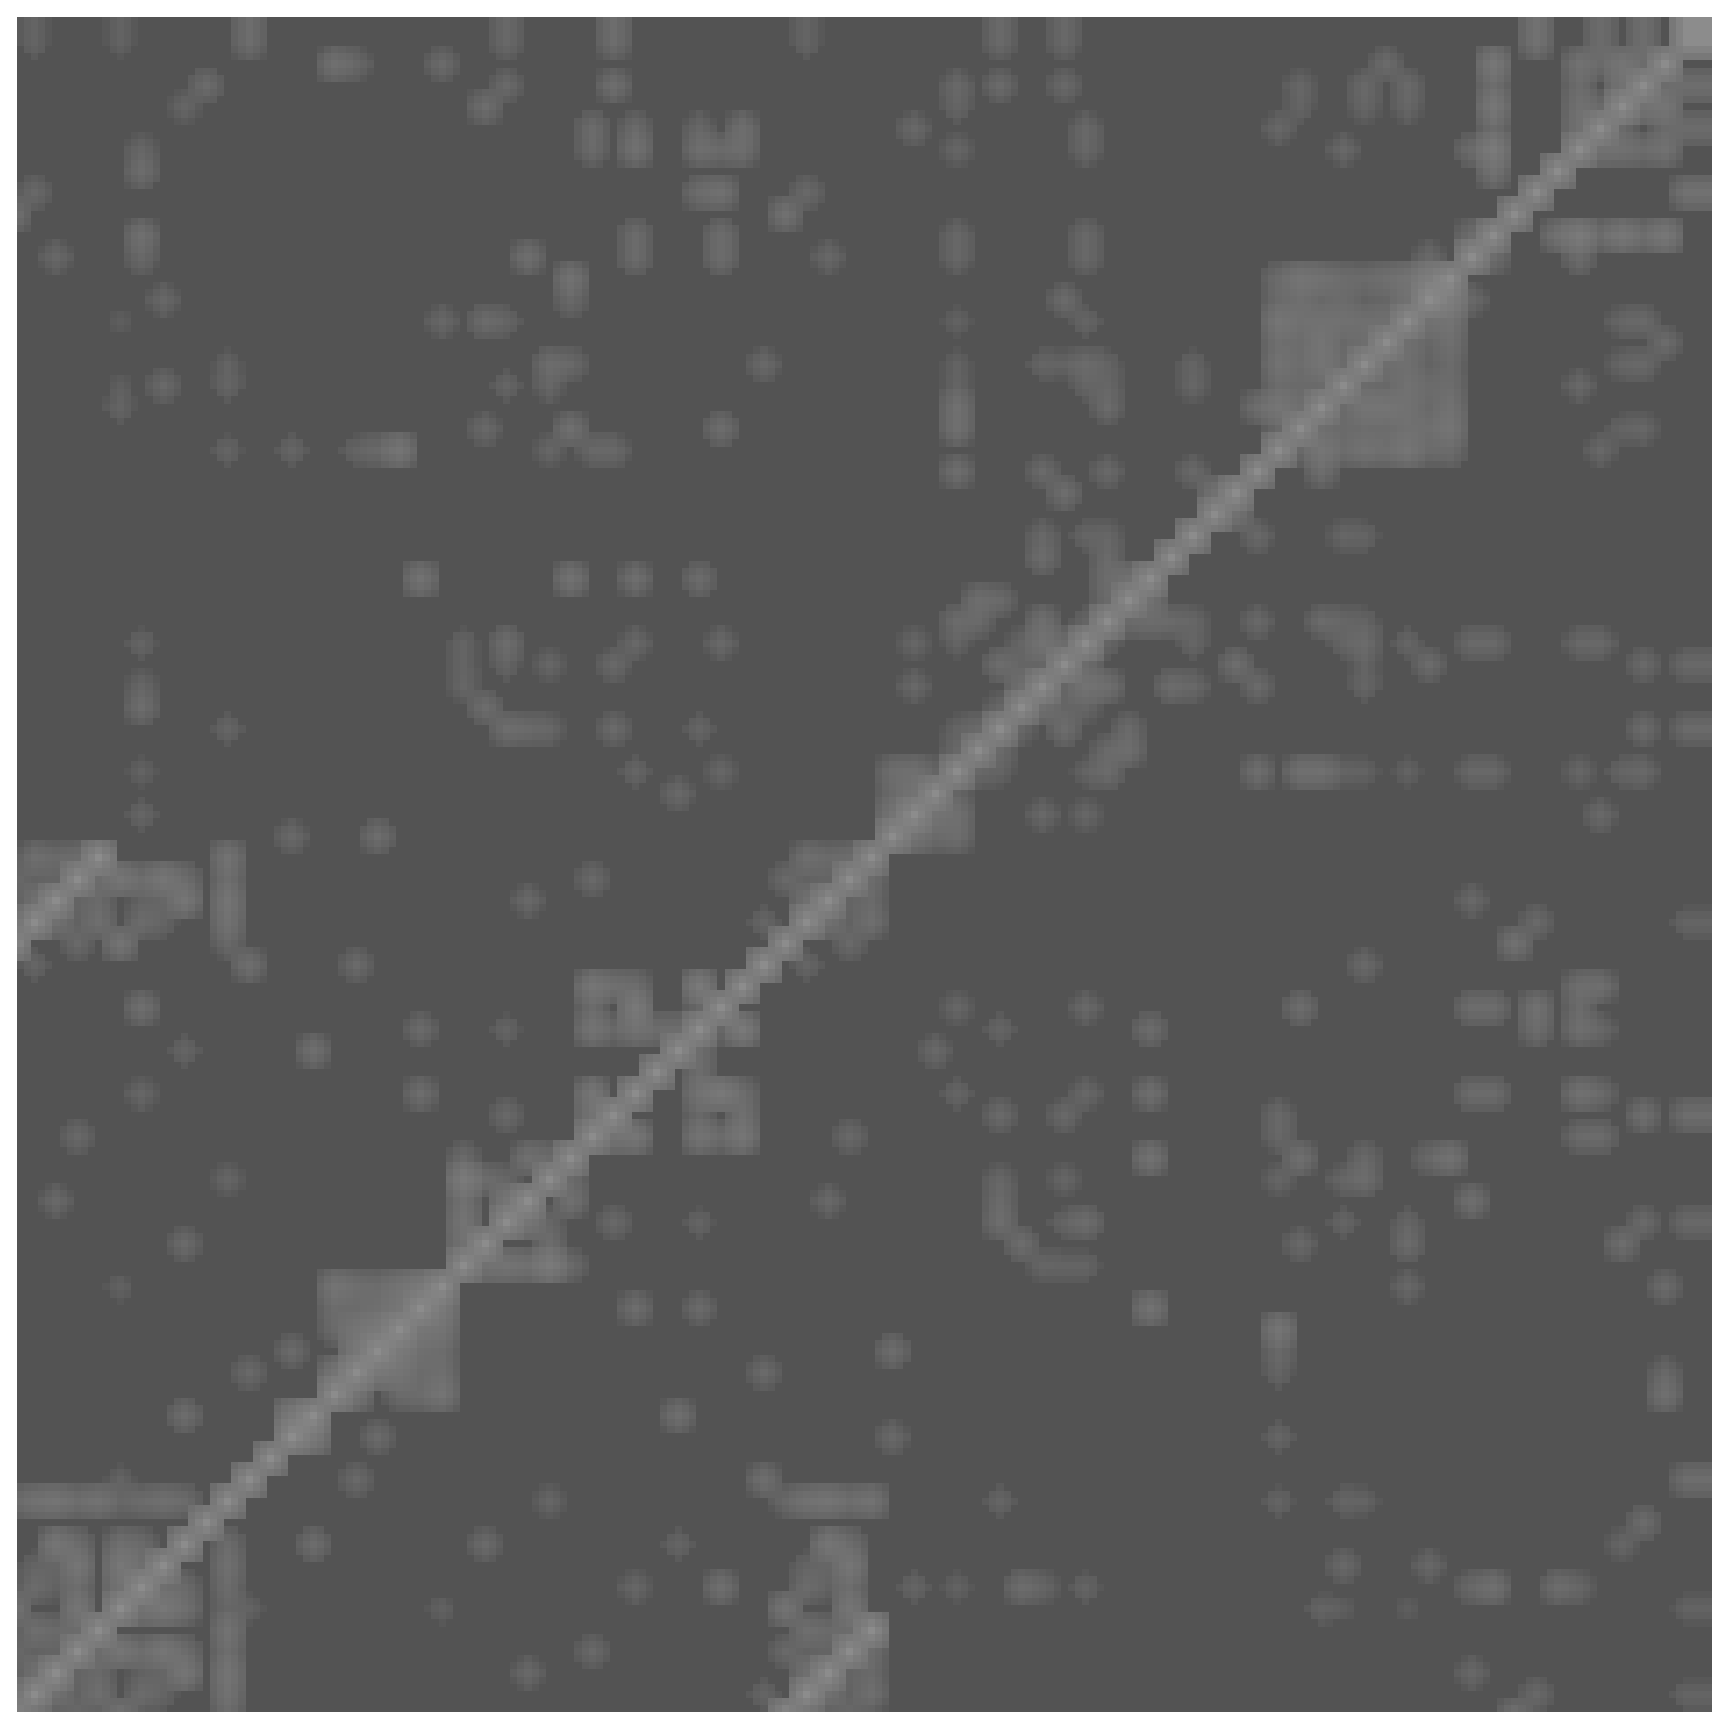
\includegraphics[width=0.3\textwidth]{simMatrix.eps}
\end{center}
\caption{An example similarity matrix.}
\label{fig:simmatrix}
\end{figure}

\subsection{Ranking}
Language usage varies throughout a document. For instance, the introduction section of a document is less cohesive than a section which is about a particular topic. Consequently, it is inappropriate to directly compare the similarity values from different regions of the similarity matrix. In non-parametric statistical analysis, one compares the {\it rank} of data sets when the qualitative behaviour is similar but the absolute quantitites are unreliable. The same idea is applied to images in computer vision to highlight local variations.

We apply the ranking scheme described in \cite{oneil_denos_1992} to the similarity matrix to eliminate the variations caused by changes in language usage. Each value in the matrix is replaced by its rank in the local region. This is obtained by counting the total number of neighbouring values it is greater than. The result is a matrix with values which relate to the statistical significance of the values in the original matrix. Figure \ref{fig:rank} shows an example of image ranking using a $3 \times 3$ rank mask. The output range is $\{0,8\}$. For segmentation we used a $11 \times 11$ rank mask with output range $\{0,120\}$.

\begin{figure}[h]
\begin{center}
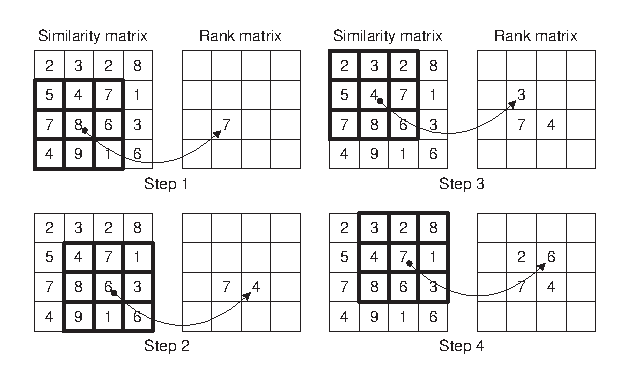
\includegraphics[width=0.48\textwidth]{ranking.eps}
\end{center}
\caption{A working example of image ranking.}
\label{fig:rank}
\end{figure}

In image processing, one tends to discard the edge and corner values where the ranking window is not contained in the image. This is unacceptable for language processing where it would involve missing out sentences. Thus, we express the rank as a proportion of the total number of neighbouring values used in the comparison for each cell to overcome this problem. To demonstrate the effect of image ranking, the process was applied to the matrix shown in figure \ref{fig:simmatrix} to produce figure \ref{fig:rankmatrix}\footnote{The process was applied to the original matrix, prior to contrast enhancement. The output image has not been enhanced.}. Notice the contrast between the dim square regions and the diagonal and off-diagonal regions in the original image has been improved significantly. Noise signals have also been reduced.

\begin{figure}[h]
\begin{center}
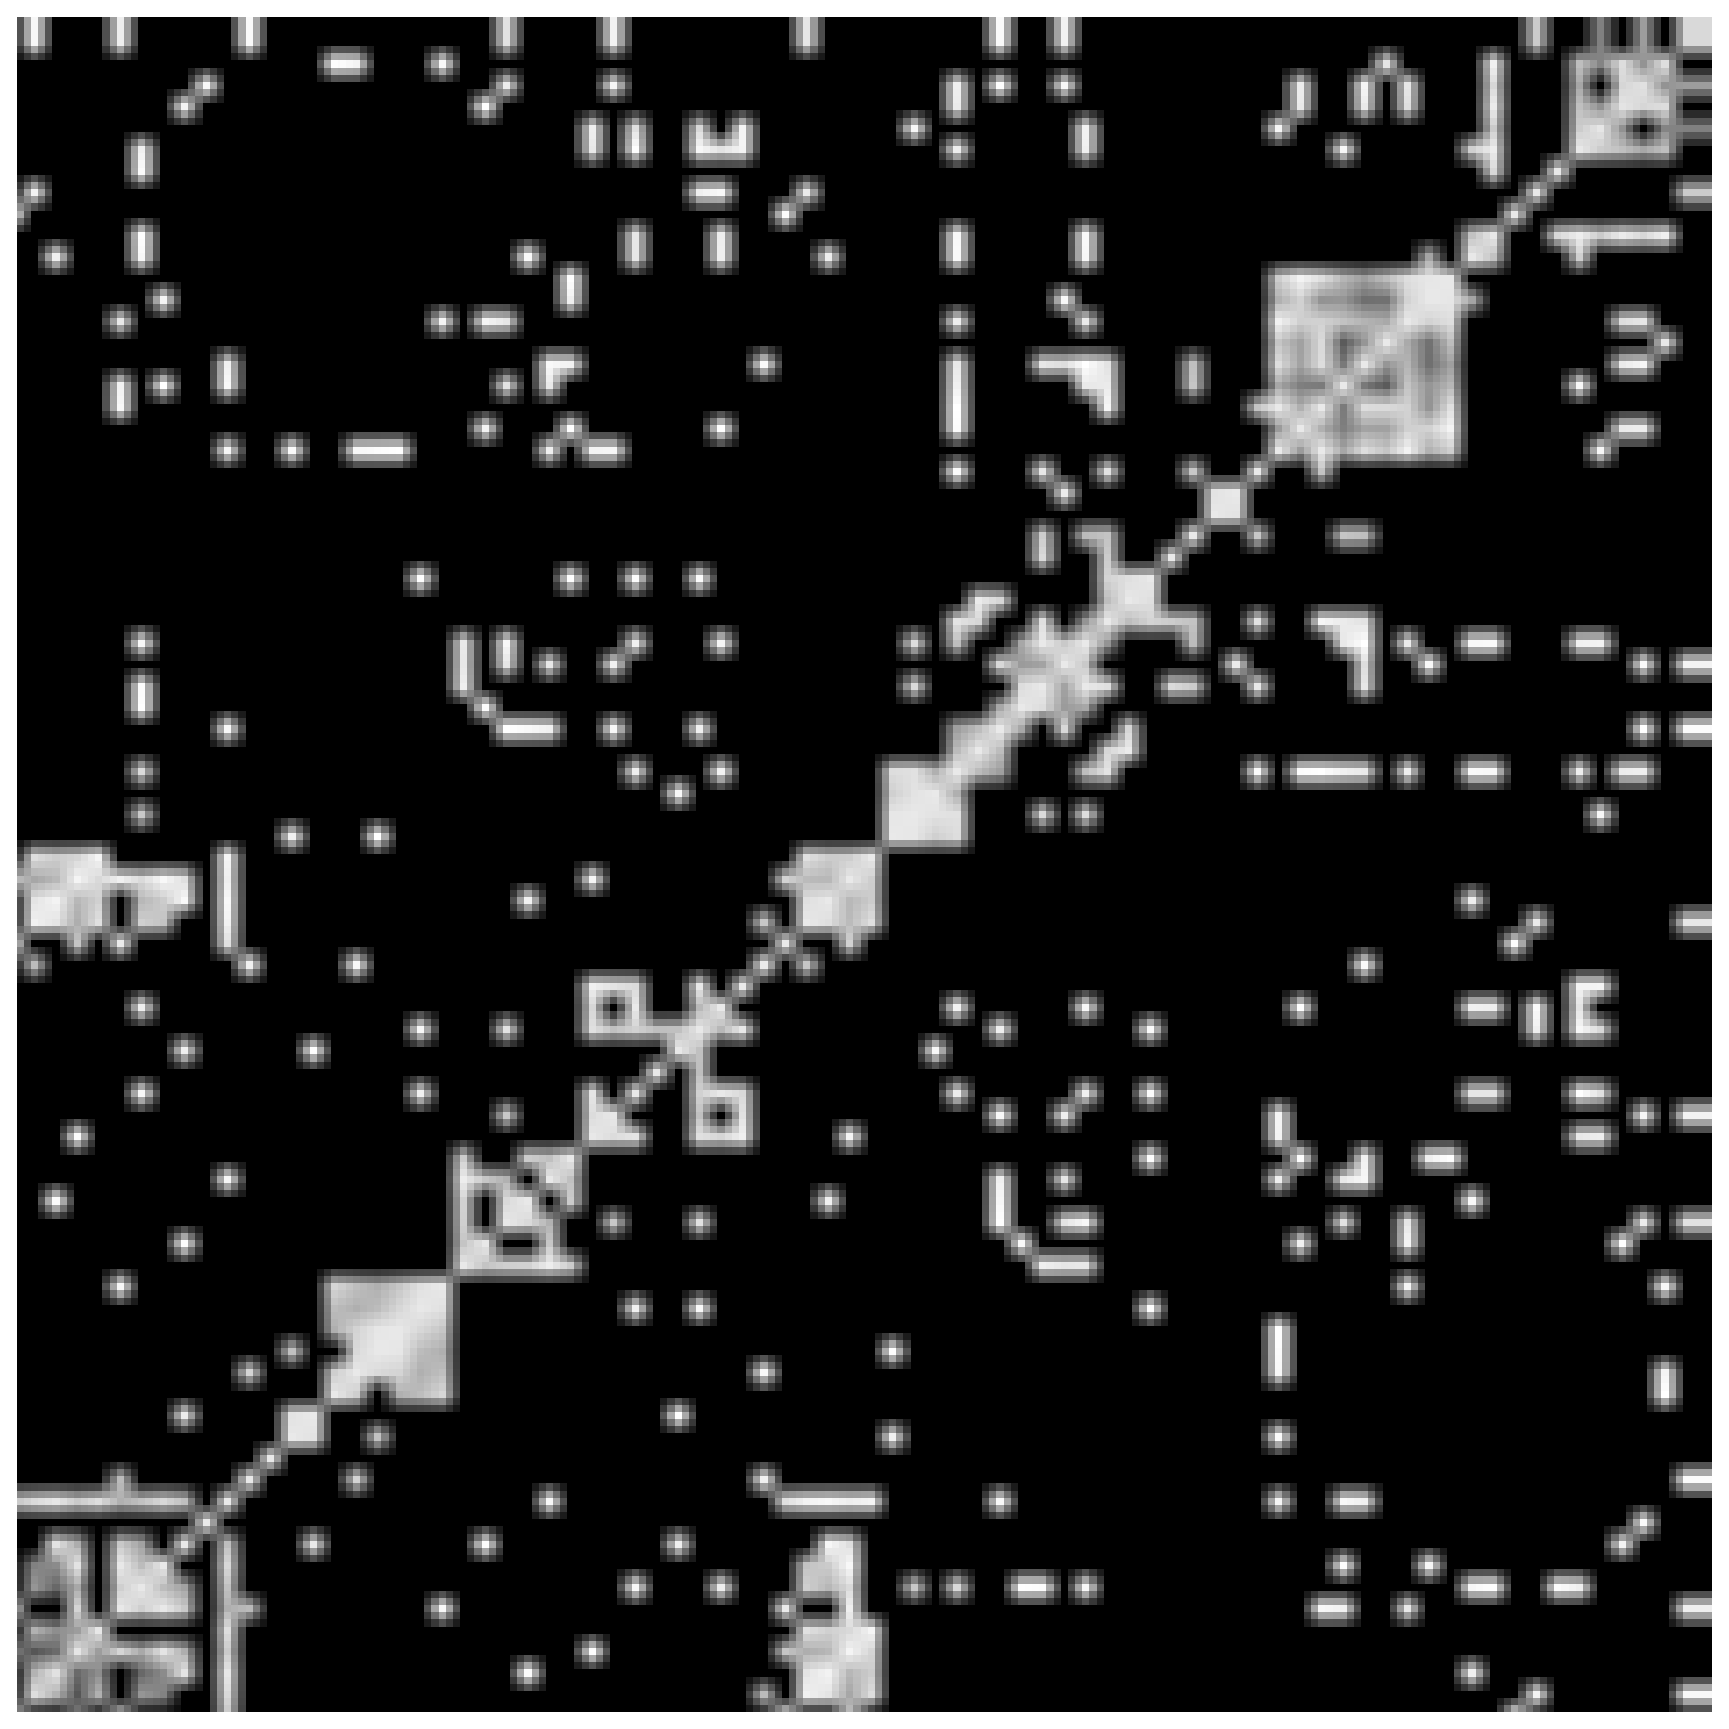
\includegraphics[width=0.3\textwidth]{rankMatrix.eps}
\end{center}
\caption{The matrix in figure \ref{fig:simmatrix} after ranking.}
\label{fig:rankmatrix}
\end{figure}

\subsection{Clustering}
The final process determines the location of the topic boundaries. The method is based on Reynar's maximization algorithm \cite{reynar_1998}. A text segment is defined by two sentences $i,j$. This is represented as a square region along the diagonal of the rank matrix. Let $s_{i,j}$ denote the sum of the rank values in a segment and $a_{i,j} = (j-i+1)^2$ be the inside area. $B = \{b_1,...,b_m\}$ is a list of $m$ coherent text segments. $s_k$ and $a_k$ refers to the sum of rank and area of segment $k$ in $B$. $D$ is the inside density of $B$ (see equation \ref{eq:insidedensity}).

\begin{equation}
D = \frac{\sum_{k=1}^{m} s_k}{\sum_{k=1}^{m} a_k}
\label{eq:insidedensity}
\end{equation}

To initialise the process, the entire document is placed in $B$ as one coherent text segment. Each step of the process splits one of the segments in $B$. The split point is a potential boundary which maximizes $D$. Figure \ref{fig:split} shows a working example. The algorithm terminates after $m-1$ steps. $m$ is either specified by the user or determined automatically by monitoring the change in density after each step, $D^{(m)} - D^{(m-1)}$.

\begin{figure}[h]
\begin{center}
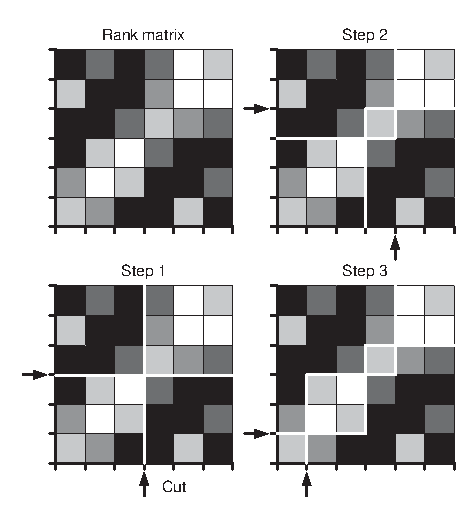
\includegraphics[width=0.48\textwidth]{clustering.eps}
\end{center}
\caption{A working example of the divisive clustering algorithm.}
\label{fig:split}
\end{figure}

The running time of each step is dominated by the computation of $s_k$. Given $s_{i,j}$ is constant, our algorithm pre-computes all the values to improve speed performance. The procedure computes the values along diagonals, starting from the main diagonal and works towards the corner. The method has a complexity of order $1\frac{1}{2} n^2$. Let $r_{i,j}$ refer to the rank value in the rank matrix $R$ and $S$ to the matrix containing all the values of $s_{i,j}$. Given $R$ of size $n \times n$, $S$ is computed in four steps (see equation \ref{eq:sumrank}). Figure \ref{fig:sumrank} shows the result of applying this procedure to the rank matrix in figure \ref{fig:split}.

\begin{equation}
\begin{array}{llcl}
1. & s_{i,i} & = & r_{i,i} \\
   &         & \textrm{for}  & i \in \{1,...,n\} \\
2. & s_{i+1,i} & = & 2 r_{i+1,i} + s_{i,i} + s_{i+1,i+1} \\
   & s_{i,i+1} & = & s_{i+1,i} \\
   &           & \textrm{for} & i \in \{1,...,n-1\} \\
3. & s_{i+j,i} & = & 2 r_{i+j,i} + s_{i+j-1,i} + \\
   &           &   & s_{i+j,i+1} - s_{i+j-1,i+1} \\
   & s_{i,i+j} & = & s_{i+j,i} \\
   &           & \textrm{for} & j \in \{2,...,n-1\} \\
   &           &   & i \in \{1,...,n-j\} \\
\end{array}
\label{eq:sumrank}
\end{equation}

\begin{figure}[h]
\begin{center}
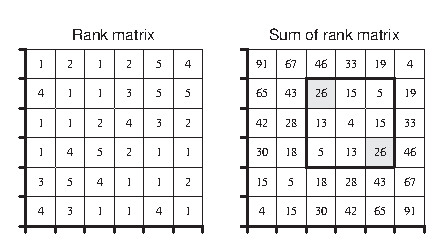
\includegraphics[width=0.48\textwidth]{ranksum.eps}
\end{center}
\caption{Improving speed performance by pre-computing $s_{i,j}$.}
\label{fig:sumrank}
\end{figure}

\section{Evaluation}
Our experiment compares the accuracy and speed performance of nine algorithms using an artificial test dataset. A test sample consists of ten text segments. A segment is the first $n$ sentences of a randomly selected document from the Brown corpus\footnote{Only the news articles {\tt ca**.pos} and informative text {\tt cj**.pos} were used in the experiment.}.

An automatic procedure generated four sets of test samples. Each set contains 50 samples and is characterised by the length of the text segments. The four sets contain segments of length between $3-5$, $6-8$, $9-11$ and $3-11$ sentences, respectively.

Accuracy is measured using the probabilistic error metric $P_D$ proposed in \cite{beeferman_et_al_1999}. Low probability indicates high accuracy. Other performance measures include the popular precision and recall metric (PR) \cite{hearst_1994}, fuzzy PR \cite{reynar_1998} and edit distance \cite{ponte_croft_1997}. The problems associated with these metrics are discussed in \cite{beeferman_et_al_1999}. Speed performance is measured by the average number of CPU seconds required to process a test sample\footnote{All experiments were conducted on a Pentium II 266MHz PC with 128Mb RAM running RedHat Linux 6.0 and the Blackdown linux port of JDK1.1.7 v3.}.

\subsection{Baseline}
Four algorithms define the baseline for the experiment. $B_n$ does not propose any boundaries. $B_a$ reports all potential boundaries as real boundaries. $B_{r,?}$ randomly selects any number of boundaries as real boundaries. $B_{r,b}$ randomly selects $b$ boundaries as real boundaries.

The accuracy of the last two algorithms is computed analytically. Given a test sample, our method computes the average probability of error over the set of all possible segmentations\footnote{The full description and explanation of the method is available from the author.}. The result of applying these four algorithms to each test data set is presented in table \ref{tbl:baseline}.

\begin{table}[ht]
\begin{center}
\begin{tabular}{|l|c|c|c|c|}
\hline
Algorithm & 3-5 & 6-8 & 9-11 & 3-11\\
\hline
$B_n$ & 0.47 & 0.47 & 0.47 & 0.46\\
$B_a$ & 0.53 & 0.53 & 0.53 & 0.54\\
$B_{r,?}$ & 0.53 & 0.53 & 0.53 & 0.54\\
$B_{r,b}$ & 0.47 & 0.47 & 0.47 & 0.46\\
\hline
\end{tabular}
\end{center}
\caption{The error rate of the baseline algorithms.}
\label{tbl:baseline}
\end{table}

\subsection{Experiment results}
Our Java implementation of four existing algorithms and our new method {\bf C99} were applied to the four test data sets. {\bf H94} represents Hearst's TextTiling algorithm \cite{hearst_1994}, {\bf K98} is Segmenter \cite{kan_et_al_1998}. We refer to Reynar's dot-plotter \cite{reynar_1998} as {\bf R98$_{max}$} (maximization) and {\bf R98$_{min}$} (minimization). The results\footnote{Some algorithms were not tested on the final data set due to their poor speed performance.} are ordered according to performance and are presented in table \ref{tbl:accuracy1} and \ref{tbl:speed1}.

\begin{table}[ht]
\begin{center}
\begin{tabular}{|l|c|c|c|c|}
\hline
Algorithm & 3-5 & 6-8 & 9-11 & 3-11\\
\hline
C99 & 0.12 & 0.09 & 0.09 & 0.11\\
R98$_{max}$ & 0.21 & 0.17 & 0.17 & 0.22\\
R98$_{min}$ & 0.34 & 0.37 & 0.37 & n/a\\
K98 & 0.44 & 0.48 & 0.51 & n/a\\
H94 & 0.46 & 0.52 & 0.53 & 0.54\\
\hline
\end{tabular}
\end{center}
\caption{The error rate of our method and four existing algorithms}
\label{tbl:accuracy1}
\end{table}


\begin{table}[ht]
\begin{center}
\begin{tabular}{|l|c|c|c|c|}
\hline
Algorithm & 3-5 & 6-8 & 9-11 & 3-11\\
\hline
H94 & 2.22 & 3.72 & 5.15 & 3.77\\
C99 & 1.91 & 3.73 & 5.99 & 3.84\\
R98$_{max}$ & 9.37 & 28.04 & 56.00 & 29.58\\
R98$_{min}$ & 19.62 & 58.77 & 122.60 & n/a\\
K98 & 21.43 & 65.54 & 129.33 & n/a\\
\hline
\end{tabular}
\end{center}
\caption{The speed performance of our method and four existing algorithms}
\label{tbl:speed1}
\end{table}

\section{Discussion}
Our experimental results show R98$_{max}$ has been the state-of-the-art. C99 out-performs R98$_{max}$ by two fold in accuracy and over seven fold in speed when used to segment the fourth dataset. The improvement is consistent over all test data sets.

Further experiments were conducted to verify the results presented in this paper. We used the same experimental procedure to compare the performance of C99 and R98$_{max}$ on another data set. The result confirms the data presented in this paper is accurate.

The speed performance test shows H94 is currently the fastest algorithm (order $n$). Although C99's performance degrades more rapidly (order $n^2$), it is over four times more accurate than H94.

Another five algorithms were developed in this work, four of which were based on C99. They applied smoothing {\bf C99s}, noise reduction {\bf C99nr} and thresholding {\bf C99t} instead of ranking to the similarity matrix. One, {\bf C99sa}, replaced the cosine similarity measure with a probabilitic measure based on spread activation over sentence vocabulary. The last algorithm {\bf K98a} is based on {\bf K98}. It uses our adaptive (rather than fixed) distance model for breaking lexical chains. These were applied to the same dataset. The results are presented in table \ref{tbl:accuracy2} and \ref{tbl:speed2}. Notice C99sa also out-performs R98$_{max}$ but the improvement is not as significant as C99. This confirms Kozima's approach \cite{kozima_1993} to computing semantic similarity does indeed improve segmentation performance. K98a is a minor improvment over K98. Details of these algorithms will be presented in a future paper. 

\begin{table}[ht]
\begin{center}
\begin{tabular}{|l|c|c|c|c|}
\hline
Algorithm & 3-5 & 6-8 & 9-11 & 3-11\\
\hline
C99sa & 0.20 & 0.14 & 0.11 & 0.18\\
C99nr & 0.19 & 0.18 & 0.19 & 0.21\\
C99t & 0.21 & 0.18 & 0.18 & 0.21\\
C99s & 0.24 & 0.20 & 0.21 & 0.24\\
K98a & 0.41 & 0.46 & 0.50 & n/a\\
\hline
\end{tabular}
\end{center}
\caption{The error rate of other algorithms developed in this work}
\label{tbl:accuracy2}
\end{table}

\begin{table}[ht]
\begin{center}
\begin{tabular}{|l|c|c|c|c|}
\hline
Algorithm & 3-5 & 6-8 & 9-11 & 3-11\\
\hline
C99t & 2.26 & 4.39 & 7.10 & 4.50\\
C99s & 2.25 & 4.39 & 7.13 & 4.52\\
C99nr & 2.28 & 4.47 & 7.28 & 4.60\\
C99sa & 7.64 & 38.16 & 113.80 & 41.02\\
K98a & 21.44 & 65.49 & 129.69 & n/a\\
\hline
\end{tabular}
\end{center}
\caption{The speed performance of other algorithms developed in this work}
\label{tbl:speed2}	
\end{table}

\section{Conclusions and future work}
This paper described a new method for domain independent linear text segmentation. The use of ranking improved the accuracy of our solution by two fold. Experimental results show the method is the state-of-the-art. Our implementation of the dot-plotting method for clustering improved the speed performance of the original approach by seven fold.

Existing algorithms were compared using the probabilistic error metric proposed in \cite{beeferman_et_al_1999} and a moderate sized artificial test data set. Results confirm Reynar's maxmization algorithm \cite{reynar_1998} has been the best algorithm for segmentation.

Other algorithms were developed in this work. Our spread activation algorithm out-performs all existing algorithms. This shows Kozima's approach \cite{kozima_1993} to computing semantic similarity improves segmentation performance.

It would be interesting to conduct the same experiment using a real data set such as the TDT3 (Topic Detection and Tracking) corpus. We would also like to compare the performance of our method with multi-source methods.

\bibliographystyle{acl}
\bibliography{references}

\end{document}
